\documentclass{paper}
\usepackage{nomencl}
\usepackage{amsmath}
\usepackage{graphicx}
\usepackage{subfigure}
\usepackage{parskip}
\usepackage[toc,page]{appendix}
\usepackage{csquotes}
\usepackage{framed}
\usepackage{amsthm}

\theoremstyle{theorem}
\newtheorem{theorem}{Theorem}[section]
 
\theoremstyle{definition}
\newtheorem{definition}{Definition}[section]

\theoremstyle{remark}
\newtheorem{remark}{Remark}[section]

\title{Kalman Filter}
\author{A. Giavaras}
\date{}

\begin{document}
\maketitle
\tableofcontents

\clearpage
\chapter{Kalman Filters}
\label{kalman_filters}

Kalman filtering is an iterative process that uses a set of equations and consecutive data inputs to quickly estimat the 
true value; e.g. position, velocity etc., of the object being measured when the measured values contain unpredicted or 
random error, uncertainty or variation.

One of the principal uses of observers in practice is to estimate the state of a
system in the presence of noisy measurements. We have not yet treated noise in our
analysis, and a full treatment of stochastic dynamical systems is beyond the scope
of this text. In this section, we present a brief introduction to the use of stochastic
systems analysis for constructing observers. We work primarily in discrete time to
avoid some of the complications associated with continuous-time random processes
and to keep the mathematical prerequisites to a minimum. This section assumes
basic knowledge of random variables and stochastic processes; see Kumar and
Varaiya [KV86] or Åström [Åst06] for the required material.

Consider again the LTI state-space model

\begin{equation}
\frac{dx}{dt} = Ax + Bu +v  ~~ y = Cx + Du +w 
\end{equation}
the model is augmented with additional terms representing the error or disturbance. Concretely,
$v$ is the process disturbance and $w$ is measurements noise. Both are assumed to be normally distibuted with zero mean;

\begin{eqnarray}
E[v] = 0, ~~ E[vv^T] = R_v, ~~ E[w] = 0, ~~ E[ww^T] = R_w 
\label{noise_proccess_1} 
\end{eqnarray}



\begin{framed}
\theoremstyle{remark}
\begin{remark}{\textbf{Normally distributed random variable}}

A one dimensional random variable $X$ is said to follow the normal distribution
\end{remark}
\end{framed}


\begin{framed}
\theoremstyle{remark}
\begin{remark}{\textbf{Nonlinear Systems}}

The definition above holds for nonlinear systems as well, and the results discussed here have extensions to the nonlinear case.
\end{remark}
\end{framed}

$R_v$ and $R_w$ are the covariance matrices for the process disturbance $v$ and the measurement noise $w$ respectively. Furthermore, we assume that the variables $v, w$ are not correlated i.e 

\begin{eqnarray}
E[vw^T] = 0
\label{noise_proccess_2} 
\end{eqnarray}


\begin{framed}
\theoremstyle{remark}
\begin{remark}{\textbf{Corralated random variables}}

Two random variables $X$ and $Y$ are said to be linearly correlated 
\end{remark}
\end{framed}

The initial condition is also modeled as a Gaussian random variable

\begin{eqnarray}
E[x(0)] = x_0, ~~ E[x(0)x^{T}(0)] = P_0
\label{noise_proccess_3} 
\end{eqnarray}

Implementation of the state-space model in a computer requires discretization. Thus the system can be written as discrete-time linear system with dynamics governed by

\begin{equation}
x_{t+1} = Ax_t + Bu_t + Fv_t,  ~~ y_t = Cx_t + w_t 
\end{equation}

Given the measurements $\{y(\tau), 0 \leq \tau \leq t \}$, we would like to find an estimate $\hat{x}_t$ that minimizes the mean square error:

\begin{equation}
E[(x_t - \hat{x}_t)(x_t - \hat{x}_t)^T] 
\end{equation}

\begin{framed}
\theoremstyle{theorem}
\begin{theorem}{\textbf{Kalman 1961}}


Consider the random process $x_t$ with dynamics described by  

\begin{equation}
x_{t+1} = Ax_t + Bu_t + Fv_t,  ~~ y_t = Cx_t + w_t \nonumber
\end{equation} 

and noise processes and initial conditions described by \ref{noise_proccess_1},  \ref{noise_proccess_2} and 
\ref{noise_proccess_3}. The observer gain $L$ that minimizes the mean square error is given by  

\begin{equation}
L_t = AP_tC^T(R_w + CP_tC^T)^{-1}  \nonumber
\end{equation}

where

\begin{equation}
P_{t+1} =  (A − LC)P_t(A − LC)^T + R_v LR_w L^T, ~~ P_0 = E[x_0x^{T}_0\}
\end{equation}

\end{theorem}
\end{framed}

A proof of this result can be found in \cite{Astrom}. We, note, however the following points:

\begin{itemize}
\item the Kalman filter has the form of a recursive filter: given mean square error $P_t$ at time $t$, we can compute how the estimate and error change. Thus we do not need to keep track of old values of the output.
\item Furthermore, the Kalman filter gives the estimate $\hat{x}_t$ and the error covariance $P_t$, so we can see how reliable the estimate is. 
It can also be shown that the Kalman filter extracts the maximum possible information about output data. 
If we form the residual between the measured output and the estimated output,
\end{itemize}

\begin{equation}
e_t = y_t - C\hat{x}_t
\end{equation}
we can show that for the Kalman filter the error covariance matrix $R_e$ is

\begin{equation}
R_e(i,j) = E(e_{j}e_{k}^{T}) = W_t\delta_{jk} 
\end{equation}

In other words, the error is a white noise process, so there is no remaining dynamic information content in the error.




\begin{framed}
\theoremstyle{theorem}
\begin{theorem}{\textbf{Kalman-Bucy 1961}}


The optimal estimator has the form of a linear observer 

\begin{equation}
\frac{d\hat{x}}{t} = A\hat{x} + Bu + L(y - C\hat{x}),  ~~ \hat{x}(0) = E(x(0)) \nonumber
\end{equation} 

where $L$ is given by

\begin{equation}
L = PC^TR_{w}^{-1}  \nonumber
\end{equation}

where $P$


\end{theorem}
\end{framed}


All matrices $A, B, C, R_v, R_w, P$ and $L$ can be time varying. The essential condition is that the Riccati equation (8.30) has a unique positive 
solution.

\section{Kalman’s Decomposition of a Linear System}

In this chapter and the previous one we have seen that two fundamental properties
of a linear input/output system are reachability and observability. It turns out that
these two properties can be used to classify the dynamics of a system. The key
result is Kalman’s decomposition theorem, which says that a linear system can be
divided into four subsystems:

\begin{itemize}
\item $\Sigma_{ro}$ which is reachable and observable
\item $\Sigma_{r\bar{o}}$ which is reachable but no observable 
\item $\Sigma_{\bar{r}o}$ which is not reachable but is observable
\item $\Sigma_{\bar{r}\bar{o}}$which is neither reachable nor observable
\end{itemize}


Thus from the input/output point of view, it is only the reachable and observable
dynamics that matter.


\begin{framed}
\theoremstyle{remark}
\begin{remark}{\textbf{Kalman's decomposition for state-space}}

The general case of the Kalman decomposition is more complica
ted and requires some additional linear algebra; see the original pap
er by Kalman, Ho, and Narendra [KHN63]. The key result is that the state space can still be decomposed
into four parts, but there will be additional coupling so that the equations have the form 
\end{remark}
\end{framed}



\section{Non-linear Filtering}
\label{non_linear_filtering}

We developed the Kalman filter algorithm using the following linear state space model

\begin{eqnarray}
\mathbf{x}_k = \mathbf{F}_{k-1}\mathbf{x}_{k-1} + \mathbf{G}_{k-1}\mathbf{u}_{k-1} + \mathbf{w}_{k-1} \\
\mathbf{y}_k = \mathbf{H}_k \mathbf{x}_k + \mathbf{v}_k
\end{eqnarray}

Using this model, we then soleved the filtering problem iteratively using a predictor-corrector type of scheme

\begin{eqnarray}
\text{Predict:}~~ p(\mathbf{x}_k|\mathbf{y}_{1:k-1}) = \int p(\mathbf{x}_k|\mathbf{x}_{k-1})p(\mathbf{x}_{k-1}|\mathbf{y}_{1:k-1}) d \mathbf{x}_{k-1} \\
\text{Update:}~~ p(\mathbf{x}_k|\mathbf{y}_{1:k}) = \frac{p(\mathbf{y}_k|\mathbf{x}_{k})p(\mathbf{x}_{k}) | \mathbf{y}_{1:k-1})}{\int p(\mathbf{y}_k|\mathbf{x}_{k})p(\mathbf{x}_{k}|\mathbf{y}_{1:k-1}) d \mathbf{x}_{k}}
\end{eqnarray}

For linear Gaussian models the Kalman filter provides and analytical solution.


\subsection{Nonlinear models}

However, many important motion and measurement models are nonlinear. For example the coordinated turn motion model is given by

\begin{eqnarray}
\begin{bmatrix}
x_k \\
y_k \\
v_k \\
\phi_k \\
\omega_k
\end{bmatrix} = 
\begin{bmatrix}
x_{k-1} + \frac{2v_{k-1}}{\omega_{k-1}}\sin(\frac{\omega_{k-1}T)}{2}\cos(\phi_{k-1} + \frac{\omega_{k-1}T}{2}) \\
y_{k-1} + \frac{2v_{k-1}}{\omega_{k-1}}\sin(\frac{\omega_{k-1}T)}{2}\sin(\phi_{k-1} + \frac{\omega_{k-1}T}{2}) \\
v_{k-1}
\phi_{k-1} + T \omega_{k-1} \\
\omega_{k-1}
\end{bmatrix} + \mathbf{q}_{k-1} \\
y_k = \sqrt{x_{k}^2 + y_{k}^2} + r_k
\end{eqnarray}

for such models we, generally, cannot obtain an anlytical solution to the filtering equations. A common approach to solve this, is to find tractable approximate solutions.


\begin{framed}
\theoremstyle{remark}
\begin{remark}{\textbf{Why is nonlinear filtering hard?}}

This is because of the following two reasons

\begin{itemize}
\item We cannot in general find an analytical solution to our filtering equations.
\item For linear systems, it is enough to describe the posterior using the first two moments, the mean and the covariance. For nonlinear systems, 
we in general need infinitely many moments to describe the true posterior.
\end{itemize}

The optimal filtering equations hold also in the non-linear setting. It is just harder to solve the equations, because we cannot find 
analytical solutions to them (in general). When the models are linear and Gaussian, the posterior density 
is also Gaussian, which means it could be described completely by the first two moments only. 
In the non-linear setting, we need infinitely many moments to fully describe the posterior, so approximations are necessary.

Weather the Markov property holds or not decides if you can at all use recursive filters to solve your estimation problem. 
In this chapter we still assume that the Markov property holds.
\end{remark}
\end{framed} 

Nonlinear filtering can be a difficult and complex subject.  It is certainly not as 
mature, cohesive, or well understood  as linear filtering. There is still a lot of  room 
for advances and improvement in nonlinear estimation techniques.  However, some 
nonlinear  estimation methods have become  (or are becoming) widespread.  These 
techniques  include nonlinear  extensions of  the Kalman filter,  unscented  filtering, 
and particle filtering. 


\section{Questions}

\begin{enumerate}
\item Which of the following statements are true?

\begin{enumerate}
\item Our choice of density parametrization will both effect the performance of our filter and the computational complexity. 
\item In real-time applications, having a recursive filter means that our compute time for producing a new estimate is more or less constant with each new measurement. 
\item In nonlinear filtering, a recursive algorithm will always find a better or equally good approximation of the true posterior as a non-recursive filter. 
\item A prerequisite for a recursive filter is that the prior and posterior density in each recursion can be described using the same density parametrization. 
\end{enumerate}
\end{enumerate}



\section{Extended Kalman Filter}
\label{extended_kalman_filter}

All of  our discussion to this point has considered linear filters for linear systems.
Unfortunately, linear systems do not  exist.  All systems are ultimately nonlinear.

However, many systems are  close enough to linear that linear estimation approaches give satisfactory results. 
But  close enough can only be carried so far.  Eventually, we run across a system 
that does not behave linearly even over a small range of  operation, and our linear 
approaches for  estimation  no longer give good results.  In this case, we  need  to  explore nonlinear estimators. 

Nonlinear filtering can be a difficult and complex subject.  It is certainly not as 
mature, cohesive, or well understood  as linear filtering. There is still a lot of  room 
for advances and improvement in nonlinear estimation techniques.  However, some 
nonlinear  estimation methods have become  (or are becoming) widespread.  These 
techniques  include nonlinear  extensions of  the Kalman filter,  unscented  filtering, 
and particle filtering.

In this section, we will discuss some nonlinear extensions of  the Kalman filter. 
The Kalman filter  that we  discussed earlier  in this book  directly  applies only to 
linear  systems.  However,  a  nonlinear  system  can  be  linearized  as discussed  in 
Section  1.3, and then  linear  estimation  techniques  (such  as the  Kalman  or  $H_{\infty}$, 
filter) can be applied.  This chapter discusses those types of approaches to nonlinear 
Kalman filtering.



\subsection{The Linearized Kalaman Filter }
In  this section, we  will show how  to linearize a nonlinear system, and  then  use 
Kalman  filtering theory to estimate the  deviations  of  the state  from a  nominal 
state value. This will then give us an estimate of the state of the nonlinear system.

We will derive the linearized Kalman filter from the continuowtime viewpoint, but 
the analogous derivation for discretetime or hybrid systems are straightforward.

\subsection{The Extended Kalaman Filter }


\section{Error State Extended Kalman Filter}
\label{error_state_extended_kalman_filter}

The previous section introduced the Extended
Kalman Filter, which uses local linearization as a way to allow us to apply the Kalman
filter equations to non-linear systems. In this section, we are going to look
at a variant of the EKF called the Error-State Extended
Kalman Filter, or ES-EKF, which has a couple of nice properties. 

By the end of this section, you should be able to describe the error state
formulation of the Extended Kalman Filter, and describe the advantages of the error state EKF
over the vanilla EKF that you learned about in the
previous video. 

The idea behind
the error state EKF is really very simple. We are going to start thinking about our vehicle state, $\mathbf{x}$, as being composed
of two parts; 

\begin{itemize}
\item A large part called the nominal state, $\hat{\mathbf{x}}$
\item A small part called the error state $\delta \mathbf{x}$
\end{itemize}

We can think of a simple example of tracking the position of a car over time. 


The green line in Figure shows the true position
of the car, which is the quantity we're trying to estimate. 


\begin{figure}[!htb]
\begin{center}
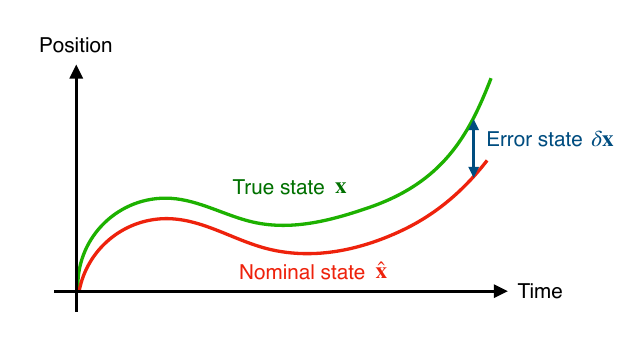
\includegraphics[scale=0.280]{img/kalman_filter/es_extended_kalman_filter_1.jpeg}
\end{center}
\caption{Summary of EKF.}
\label{es_extended_kalman_filter_1}
\end{figure}

The red line is the nominal state, or our best guess what the true state could
be based on what we know about the car's motion model and acceleration and breaking inputs. 

Of course, our motion model is never perfect, and there is always some random process noise. These errors build up over time as we integrate
the motion model. We can think of the error state as the place where all of these modelling errors and process noise
accumulate over time, so that the error state is just the difference between the nominal state and the true state at any given time. 
If we can figure out what the error state is, we can actually use it as a correction to the nominal state to bring us closer to
the true state. 

So, in the error state EKF, instead of doing Kalman filtering on the full state
which might have lots of complicated non-linear behaviors, we are going to
use the EKF to estimate the error
state instead, and then use the estimate of the error state as a correction to
the nominal state. 

What this means mathematically is that we are going to rearrange our
linearized motion model so that we now have an equation
that can tell us how the difference between the true state at time, $k$, and our predicted
state at time, $k$, is related to
the same difference at time, $k-1$. These differences
are exactly the error states we just talked about; $\delta \mathbf{x}_k$  and
$\delta \mathbf{x}_{k-1}$, and the equations relating them are called the error
state kinematics. We can also re-express our linearized
measurement model in terms of the error state directly. We can use this error state formulation of the EKF in
a very similar way to the vanilla EKF. 

We start off by updating the nominal state using the non-linear motion model and our current best
estimate of the state. We could do this a bunch of times before ever getting a measurement for the correction step. So, the current
best estimate might be $\chek{\mathbf{x}}$ or $\hat{\mathbf{x}}$. We also need to keep track of the state covariance, which grows as
we integrate more and more process noise from the motion model. Note that again, the previous
covariance estimate could be $\chek{\mathbf{P}}$  or $\hat{\mathbf{P}}$ depending
on whether we used a measurement to do a correction step. We can repeat the loop updating the
nominal state and the error state covariance for as long as we like until we receive
the measurement and want to do a correction. When this happens, we can compute the Kalman gain as usual, and then compute
the best estimate of the error state using
the Kalman gain, the measurement, and our nonlinear
measurement model. 

Once we have an estimate for the mean of
the error state, we want to use this to update the nominal state and
correct the error. We can do that by just adding our estimate
of the error state to the nominal state to get the correct state estimate for the full state. 
Finally, we can update the state covariance using the usual equations.

This process goes on forever, or at least until the vehicle runs out of gas. So, why would we
actually want to use the error state EKF
in practice? Well, there are two
good reasons to use it. 

\begin{itemize}
\item One reason is that it can often work better than the vanilla EKF because the small error
state is more amenable to
linear filtering than the large
nominal state, which we can integrate
non-linearly. 
\item The other reason is that the error state
formulation makes it much easier to work with constrained quantities like rotations, which
will come in handy a bit later in the course. The reason for
this is that we don't necessarily have to use plane vector addition to break down the state. In fact, we could use any generalized
composition operation we like as long as it gives us a consistent way
of incorporating small perturbations
into the nominal state. 
\end{itemize}

If this all sounds a bit abstract right now, don't worry. Later in the
course, we'll use the error state
EKF to help us deal with rotations
in 3D space, which are
a very common type of constraint quantity. 

In summary, the error state formulation of the EKF separates the vehicle state into a large nominal state and a small error state. The nominal state
keeps track of what the motion model predicts the states should be, while the error state captures the
modelling errors and process noise that accumulate over time. In the error state EKF, we estimate
this small error state and use it as a correction to the nominal state. This is the main
difference between the error state EKF and the vanilla EKF, which estimates the full state. Keep in mind that both formulations still rely on
local linearization. The error state EKF has a couple of advantages over the vanilla EKF. The first is that it simply performs better because
the evolution of the error state tends to be closer to linear. The other is that the error state
formulation makes it easier to handle special quantities
like 3D rotations. 
\section{Questions}
\section{Assignements}

\section{Unscented Kalman Filter}
\label{unscented_kalman_filter}

In the previous section, we saw how linearization errors can cause the EKF to produce state estimates that are very different from
the true value of the state and produce covariances that don't accurately
capture the uncertainty in the state. This can be a big problem when we're relying on the EKF in safety critical applications
like self driving cars. In this section, we will discuss the Unscented Kalman
Filter, which is an alternative approach to nonlinear Kalman filtering that
relies on something called the unscented transform to pass probability
distributions through nonlinear functions. As we will see, the unscented transform
gives us much higher accuracy than analytical EKF style linearization,
for a similar amount of computation, and without needing to compute any Jacobians. 

Hence, by the end of this section, you will be able to use the unscented transform to pass a probability distribution
through a nonlinear function. Describe how the Unscented Kalman Filter, or UKF, uses the unscented transform in
the predication and correction steps. And explain the advantages
of the UKF over the EKF, as well as apply the UKF to a simple
nonlinear tracking problem. 

\section{The unscented transform}
\label{unscented_transform}

The intuition behind the unscented
transform is simple. It's typically much easier to approximate a probability distribution than it is to approximate an arbitrary
nonlinear functions. Let's see  a simple example where a 1D Gaussian distribution like the one on shown on Figure, gets transforms
to a nonlinear function into a more complicated a 1D distribution
like the one on the right. 

\begin{figure}[!htb]
\begin{center}
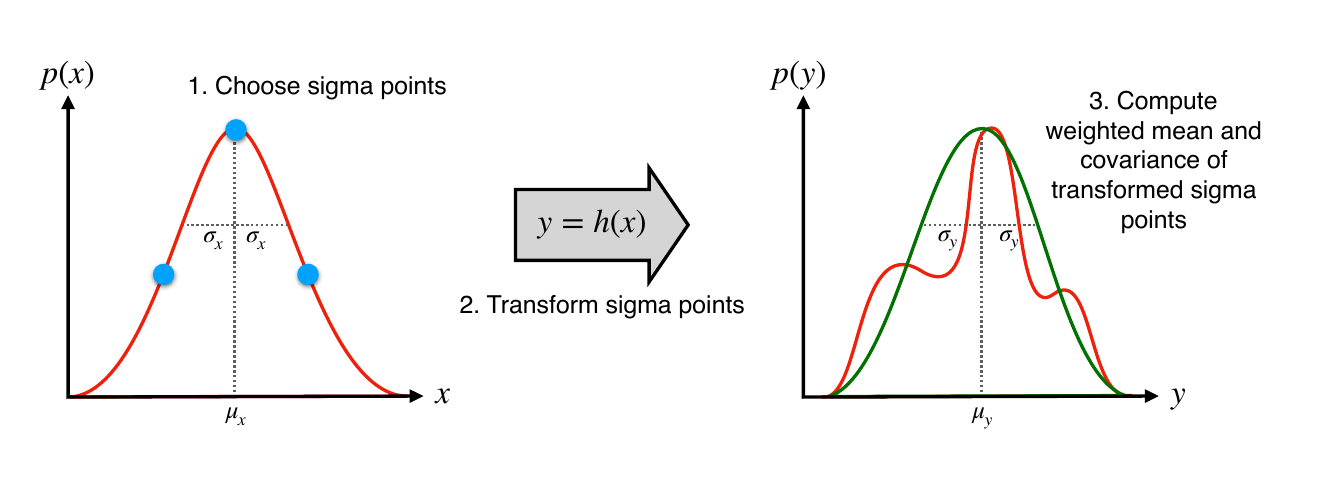
\includegraphics[scale=0.280]{img/kalman_filter/unscented_kalman_filter_1.jpeg}
\end{center}
\caption{Summary of EKF.}
\label{unscented_kalman_filter_1}
\end{figure}

We already know the mean and standard deviation of the input Gaussian, and we want to figure out the mean and
standard deviation of the output distribution using this information and
the nonlinear function. The unscented transform
gives us a way to do this. The basic idea in the unscented
transform has three steps. 

\begin{itemize}
\item We choose a set of sample points from our input distribution. These are not random samples,
they are deterministic samples, chosen to be a certain number of standard deviations away from the mean. For this reason,
these samples are called sigma points and the unscented transform is sometimes
called the sigma point transform. 
\item Once we have our set of carefully chosen sigma points, the second and easiest step is to pass each sigma point
to our nonlinear function producing a new set of sigma points belonging to the output distribution. 
\item Finally, we can compute the sample mean and covariance of the output sigma points with some carefully chosen weights, and
these will give us a good approximation of the mean and covariance of the true output distribution. 
\end{itemize}

Now, that we have seen the basic
idea of the unscented transform, let's look at each of these steps in detail. 

The first thing you might be wondering is, how many sigma points do we need and which points are in fact sigma points? In general, for
an $N$-dimensional probability distribution $N(\mu, \Sigma)$, we need $2N + 1$ sigma points. One for the mean, and the rest
symmetrically distributed about the mean. The diagrams on the left show the sigma
points for one dimensional and two dimensional examples. 

\begin{figure}[!htb]
\begin{center}
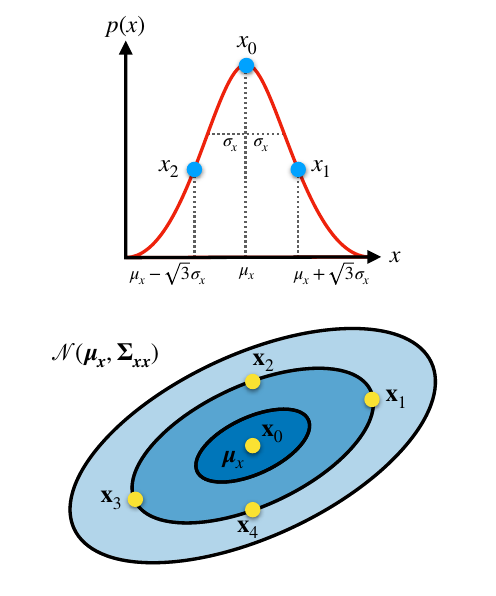
\includegraphics[scale=0.280]{img/kalman_filter/unscented_kalman_filter_2.jpeg}
\end{center}
\caption{Summary of EKF.}
\label{unscented_kalman_filter_2}
\end{figure}

In 1D, we need two sigma points, and in 2D, we need five. The first step in determining where
the sigma point is taking something called the Cholesky decomposition
of the covariance matrix associated with the input distribution. The Cholesky decomposition is basically
a square root operation that operates on symmetric positive definite matrices,
such as covariance matrices. 


\begin{equation}
\Sigma = LL^T
\end{equation}

where $L$ is a lower triangular matrix.

\begin{framed}
\theoremstyle{remark}
\begin{remark}{\textbf{Cholesky Decomposition}}

\end{remark}
\end{framed}

In fact, if the input PDF is one dimensional, the Cholesky decomposition really is
just the square root of the variance which is also known as
the standard deviation. We will not go into the details of how
to compute a Cholesky decomposition. 

Once we have decomposed the covariance matrix, we can choose our first sigma point to
be the mean of the distribution and the remainder to be the mean plus or
minus some factor times each column of the matrix $L$ that
we got from the Cholesky decomposition. 

\begin{eqnarray}
\mathbf{x}_0 = \boldsymbol{\mu} \\
\mathbf{x}_i = \boldsymbol{\mu} + \sqrt{N + \kappa} \text{col}_i L, ~~ i = 1, \ldots, L
\end{eqnarray}

The value of $N$ here again is the number of dimensions of the probability distribution. The parameter $\kappa$ is a tuning parameter
that you're free to set yourself. For Gaussian distributions, which is what we will be working with, setting $N + \kappa$ equal
to three is a good choice. 

\begin{eqnarray}
\mathbf{x}_{i + N} = \boldsymbol{\mu} - \sqrt{N + \kappa} \text{col}_i L, ~~ i = 1, \ldots, L, \kappa = 3 - N
\end{eqnarray}

So now we have our set of sigma points. The next step is straight forward, just
pass each of the sigma points through our nonlinear function $\mathbf{h}(\mathbf{x})$ to get a new
set of transform sigma points. Now all that is left is to recombine the transform sigma points to find our output mean and
output covariance. We do this using the standard formulas for the sample mean and covariance that you would have seen in you introductory statistics courses. 


\begin{eqnarray}
\boldsymbol{\mu} = \sum_{i=0}^{2N} \alpha_i \mathbf{y}_i \\
\Sigma = \sum_{i=0}^{2N} \alpha_i (\mathbf{y}_i - \boldsymbol{\mu})(\mathbf{y}_i - \boldsymbol{\mu})^T \\
\alpha_i = 
\begin{cases}
\frac{\kappa}{N + \kappa}, i =0 \\
\frac{1}{2}\frac{1}{N + \kappa}, \text{otherwise}
\end{cases}
\end{eqnarray}


The trick is that each of the points gets a specific weight in the mean and covariance calculations, and that weight
depends on the parameter $\kappa$ and the dimension of the input distribution $N$. 

\section{Unscented Kalman filter example}

To see the unscented transform in action, let get back to our example
from the Extended Kalman Filter. Where we nonlinearly transformed a uniform
distribution in polar coordinates into Cartesian coordinates. Let us see how the unscented
transform compares to the analytical linearization approach. 

So here again, we have the true mean and covariance of the two
distributions in green. Now let's apply the unscented transform. 


\begin{figure}[!htb]
\begin{center}
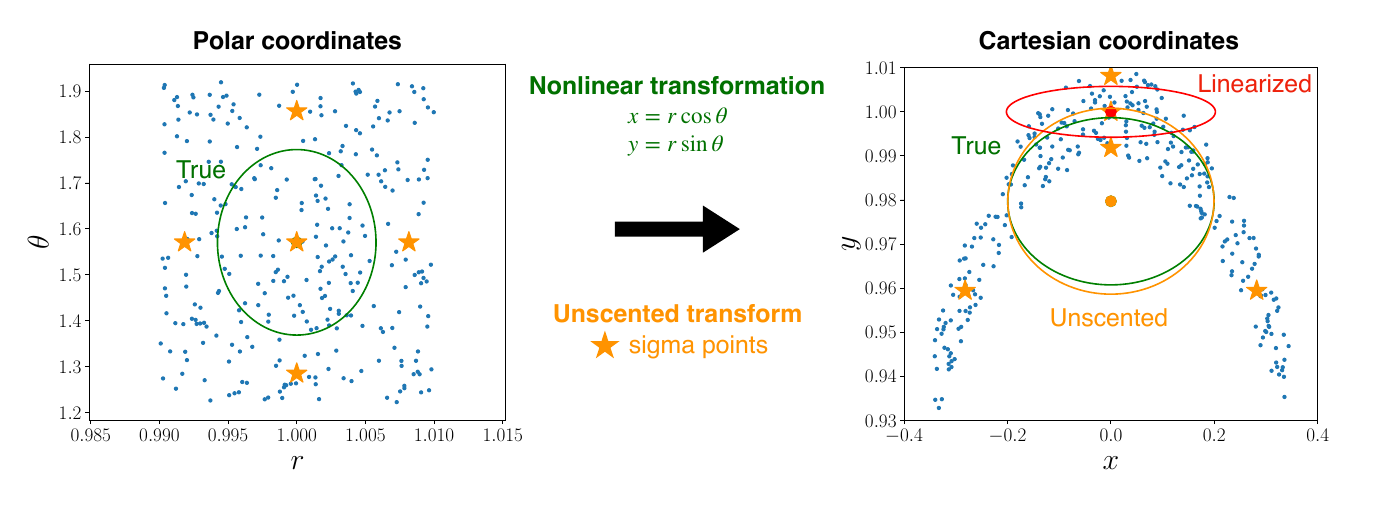
\includegraphics[scale=0.280]{img/kalman_filter/unscented_kalman_filter_3.jpeg}
\end{center}
\caption{Summary of EKF.}
\label{unscented_kalman_filter_3}
\end{figure}

The dimension of our input distribution is two so we need five sigma points which
we have shown as orange stars. Passing these sigma points to our
nonlinear function puts them here. The mean and covariance we compute
from the transformed sigma points look like this shown in orange. Note that our estimate for
the mean using the unscented transform is almost exactly the same as
the true nonlinear mean. Our estimate for the covariance almost
exactly matches the true covariance. Compare that to the analytically
linearized transformed mean and covariance in red, which are both very different
from the true mean and true covariance. It is easy to see from this example
the unscented transform gives us some much better approximation of the output
PDF without requiring much more work than the analytical
linearization approach. 

\section{Implementation}

Now that we have seen how the unscented transform works, we can easily use it in our Kalman filtering framework
to work with nonlinear models. 

\begin{eqnarray}
\mathbf{x}_k  = \mathbf{f}_{k-1}(\mathbf{x}_{k-1}, \mathbf{u}_{k-1}, \mathbf{w}_{k-1}), \mathbf{w}_{k} \sim N(\mathbf{0}, \mathbf{Q}_k)  \\
\mathbf{y}_k  = \mathbf{h}_{k}(\mathbf{x}_{k}, \mathbf{v}_{k}),  \mathbf{v}_{k} \sim N(\mathbf{0}, \mathbf{R}_k)  
\end{eqnarray}

This variant of the Kalman filter is called the Unscented Kalman Filter or UKF. You may also hear it called
the sigma point Kalman filter. The main idea of the UKF is that instead
of approximating the system equations by linearizing them, like the EKF does. We use the unscented transform to
approximate the PDFs directly. 

Let's look at the prediction step of the UKF.  In order to propagate the state and covariance
through the motion model from time $k-1$ to time $k$, we apply the unscented transform
using the current best guess for the mean and covariance of the state. First, we decompose the estimated state
covariance from time $k-1$, then we calculate our sigma points centered around
the estimated mean state from time $k-1$. Second, we propagate our sigma points
through our nonlinear motion model to get a new set of sigma points for
the predicted state at time $k$. Finally, we calculate
the predicted mean and covariance for the state at time $k$. At this point,
it is important to account for the process noise by adding its covariance
to the covariance of the transformed sigma points to get the final
predicted covariance.

\begin{itemize}
\item Compute sigma points
\end{itemize}

\begin{eqnarray}
\check{\mathbf{L}}_{k-1}\check{\mathbf{L}}_{k-1}^T  = \hat{\mathbf{P}}_{k-1}  \\
\hat{\mathbf{x}}_{k-1}^{0}  = \hat{\mathbf{x}}_{k-1} \\
\hat{\mathbf{x}}_{k-1}^{i}  = \hat{\mathbf{x}}_{k-1} + \sqrt{N + \kappa} \text{col}_i \check{\mathbf{L}}_{k-1}, i = 1, \ldots, N \\
\hat{\mathbf{x}}_{k-1}^{i + N}  = \hat{\mathbf{x}}_{k-1} - \sqrt{N + \kappa} \text{col}_i \check{\mathbf{L}}_{k-1}, i = 1, \ldots, N 
\end{eqnarray}

\begin{itemize}
\item Propagate sigma points
\end{itemize}

\begin{eqnarray}
\check{\mathbf{x}}_{k}^{i} = \mathbf{f}_{k-1}(\hat{\mathbf{x}}_{k-1}^{i}, \mathbf{u}_{k-1}, \mathbf{0}), i =0, \ldots 2N 
\end{eqnarray}

\begin{itemize}
\item  Compute predicted mean and covariance
\end{itemize}

\begin{eqnarray}
\alpha_i = 
\begin{cases}
\frac{\kappa}{N + \kappa}, i = 0 \\
\frac{1}{2}\frac{1}{N + \kappa}, \text{otherwise}
\end{cases} \\
\check{\mathbf{x}}_k = \sum_{i=0}^{2N} \alpha_i \check{\mathbf{x}}_{k}^{i} \\
\check{\mathbf{P}}_k = \sum_{i=0}^{2N} \alpha_i (\check{\mathbf{x}}_{k}^{i} - \check{\mathbf{x}}_{k})(\check{\mathbf{x}}_{k}^{i} - \check{\mathbf{x}}_{k})^T + \mathbf{Q}_{k-1}
\end{eqnarray}

This equation looks a bit different if the process noise is not additive. But most of the time, we will be dealing
with additive noise in your models unless there's a good reason not to. For the correction step,
we are going to follow a similar procedure, this time with a nonlinear measurement model. First, we will need to redraw our sigma
points using the predicted covariance matrix. We need to do this a second time
because we added process noise at the end of the last step. This will modify the positions
of some of the sigma points. Next, we are going to plug these new sigma points one by one into our nonlinear measurement model to get
another set of sigma points for the predicted measurements. Then we can estimate the mean covariance
of the predicted measurements using the sample mean and covariance formulas. 

Again, take note that we are adding in
the measurement noise covariance to get the final covariance of
the predicted measurements. Also note that this formula only applies to additive noise. In order to compute the Kalman gain, we are also
going to need the cross covariance between the predicted state and
the predictive measurement which tells us how the measurements are correlated with the state. You can calculate this using the standard
formula for the cross-covariance and using the same weights as before. Then all that is left is to use the Kalman
gain to optimally correct the mean and covariance of the predicted states,
and that's it. The UKF follows the same prediction correction pattern as the EKF, but we have just replaced the analytical linearization
step with the unscented transform. The above is summarized in Figure \ref{unscented_kalman_filter_4}

\begin{figure}[!htb]
\begin{center}
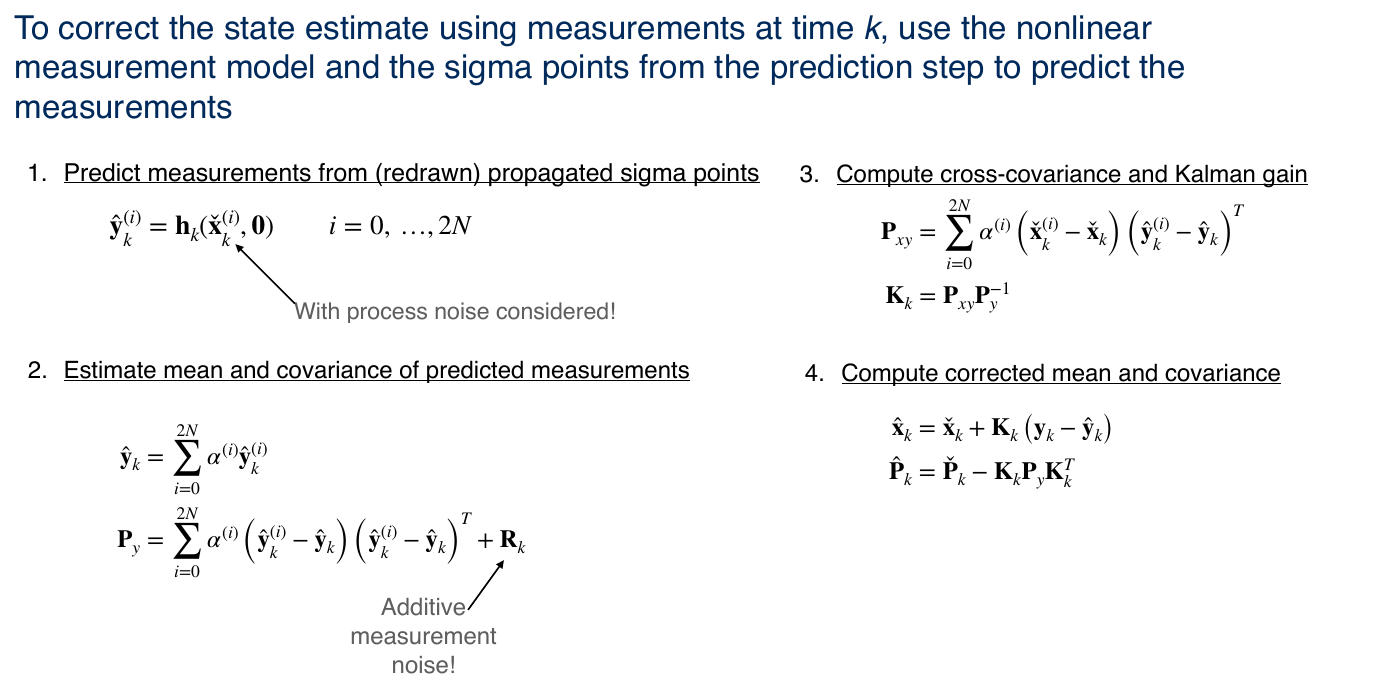
\includegraphics[scale=0.280]{img/kalman_filter/unscented_kalman_filter_4.jpeg}
\end{center}
\caption{UKF correction step.}
\label{unscented_kalman_filter_4}
\end{figure}

\section{UKF example}

Let's try applying the UKF to the same example driving scenario we worked through with the EKF. We are again trying to track the position
and velocity of a moving car that we're controlling by pressing
on the gas pedal or the brake. The car has a sensor onboard that measures
the angle between a distant landmark and the horizon. 

\begin{figure}[!htb]
\begin{center}
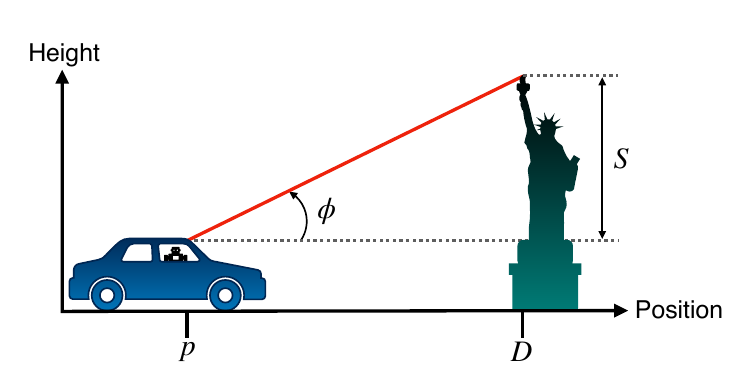
\includegraphics[scale=0.280]{img/kalman_filter/unscented_kalman_filter_5.jpeg}
\end{center}
\caption{UKF example setting.}
\label{unscented_kalman_filter_5}
\end{figure}

The motion model is linear 

\begin{eqnarray}
\mathbf{x}_k = 
\begin{bmatrix}
1 & \Delta t \\
0 & 1
\end{bmatrix}
\mathbf{x}_{k-1} + 
\begin{bmatrix}
 0 \\
 \Delta t 
\end{bmatrix}
\mathbf{u}_{k-1} + \mathbf{w}_{k-1}
\end{eqnarray}

but the measurement model is nonlinear. 

\begin{equation}
y_k = \arctan(\frac{S}{D - p_k}) + v_k
\end{equation}

Finally, we will use the following noise densities

\begin{equation}
v_k \sim N(0, 0.01), ~~ \mathbf{w}_k \sim N(\mathbf{0}, \begin{bmatrix} 0.1 & 0 \\ 0 & 0.1 \end{bmatrix})
\end{equation}

Try using the data given in equation \ref{ukf_example_data} to estimate
the position of the vehicle at time one using the UKF. 

\begin{equation}
S = 20m, D= 40m, y_1 = 30 deg, u_0 = -2m/s^2, \Delta t = 0.5s
\label{ukf_example_data}
\end{equation}

Here is the Cholesky decomposition of
the initiate covariance matrix and the five sigma points we'll use to
represent the state and its covariance. 

\begin{eqnarray}
\hat{\mathbf{L}}_0\hat{\mathbf{L}}_{0}^T = \hat{\mathbf{P}}_0 \\
\begin{bmatrix}
0.1 & 0 \\
0 & 1
\end{bmatrix}
\begin{bmatrix}
0.1 & 0 \\
0 & 1
\end{bmatrix}^T = 
\begin{bmatrix}
0.01 & 0 \\
0 & 1
\end{bmatrix}
\label{ukf_example_data}
\end{eqnarray}


\begin{eqnarray}
\hat{\mathbf{x}}_{0}^{(0)} = 
\begin{bmatrix}
0 \\
5 
\end{bmatrix} \\ 
\hat{\mathbf{x}}_{0}^{(1)} = 
\begin{bmatrix}
0 \\
5 
\end{bmatrix} + \sqrt{3} 
\begin{bmatrix}
0.1 \\
0 
\end{bmatrix} =
\begin{bmatrix}
0.2 \\
5 
\end{bmatrix} \\
\hat{\mathbf{x}}_{0}^{(2)} = 
\begin{bmatrix}
0 \\
5 
\end{bmatrix} + \sqrt{3} 
\begin{bmatrix}
0 \\
1 
\end{bmatrix} =
\begin{bmatrix}
0 \\
6.7 
\end{bmatrix} \\
\hat{\mathbf{x}}_{0}^{(3)} = 
\begin{bmatrix}
0 \\
5 
\end{bmatrix} - \sqrt{3} 
\begin{bmatrix}
0.1 \\
0 
\end{bmatrix} =
\begin{bmatrix}
-0.2 \\
5
\end{bmatrix} \\
\hat{\mathbf{x}}_{0}^{(4)} = 
\begin{bmatrix}
0 \\
5 
\end{bmatrix} - \sqrt{3} 
\begin{bmatrix}
0 \\
1 
\end{bmatrix} =
\begin{bmatrix}
0 \\
3.3
\end{bmatrix} 
\label{ukf_example_data}
\end{eqnarray}


The result of the prediction step for the mean of the state. 

\begin{eqnarray}
\check{\mathbf{x}}_{1}^{(0)} = 
\begin{bmatrix}
2.5 \\
4 
\end{bmatrix} \\ 
\check{\mathbf{x}}_{1}^{(1)} =  
\begin{bmatrix}
2.7 \\
4 
\end{bmatrix} 
\check{\mathbf{x}}_{1}^{(2)} = 
\begin{bmatrix}
3.4 \\
5.7 
\end{bmatrix} \\
\check{\mathbf{x}}_{1}^{(3)} = 
\begin{bmatrix}
2.3 \\
4
\end{bmatrix} \\
\check{\mathbf{x}}_{1}^{(4)} = 
\begin{bmatrix}
1.6 \\
2.3
\end{bmatrix} 
\label{ukf_example_prediction}
\end{eqnarray}


\begin{equation}
\check{\mathbf{x}}_k = \sum_{i=0}^{2N}\alpha_i \check{\mathbf{x}}_{k}^{(i)} = \frac{1}{3} \begin{bmatrix}
2.5 \\
4
\end{bmatrix} + \ldots + \frac{1}{6}
\begin{bmatrix}
1.6 \\
2.3
\end{bmatrix} =
\begin{bmatrix}
2.5 \\
4
\end{bmatrix}
\end{equation}

And finally, the predicted covariance. 

\begin{equation}
\check{\mathbf{P}}_k = \sum_{i=0}^{2N} \alpha_i (\check{\mathbf{x}}_{k}^{i} - \check{\mathbf{x}}_{k})(\check{\mathbf{x}}_{k}^{i} - \check{\mathbf{x}}_{k})^T + \mathbf{Q}_{k-1} =
\begin{bmatrix}
0.36 & 0.5 \\
0.5 & 1.1
\end{bmatrix}
\end{equation}
\begin{framed}
\theoremstyle{remark}
\begin{remark}{}

Notice that the predicted mean and
covariance are identical to what we would've found with the linear Kalman
filter and the extended Kalman filter.  This is because the motion
model actually is linear.
\end{remark}
\end{framed}

For the correction step, these are the sigma points for the predicted measurements and the mean
and covariance of that distribution. 


And finally,
the cross-covariance Kalman gain, and our final answer for
the position of the vehicle at time $k = 1$. 

\begin{equation}
\hat{y}_{1}^{i} = h_1(\check{\mathbf{x}}_{1}^{i}, 0), i = 0, \ldots, 2N
\end{equation}

This gives us

\begin{eqnarray}
\hat{y}_{1}^{(0)} = \arctan(\frac{20}{40 - 2.5}) = 28.1 \\ 
\hat{y}_{1}^{(1)} = \arctan(\frac{20}{40 - 2.7}) = 28.7 \\ 
\hat{y}_{1}^{(2)} = \arctan(\frac{20}{40 - 2.5}) = 28.1 \\
\hat{y}_{1}^{(3)} = \arctan(\frac{20}{40 - 2.3}) = 27.4 \\
\hat{y}_{1}^{(4)} = \arctan(\frac{20}{40 - 2.5}) = 28.1 
\label{ukf_example_prediction}
\end{eqnarray}


\begin{equation}
\hat{y}_1 = \sum_{i=0}^{2N} \alpha_i \hat{y}_{1}^{i}  = 28.1
\end{equation}

\begin{equation}
P_y = \sum_{i=0}^{2N} \alpha_i (\hat{y}_{1}^{i} -\hat{y}_{k})(\hat{y}_{1}^{i} -\hat{y}_{k})^T + R_k = 0.16
\end{equation}

\begin{equation}
\mathbf{P}_{xy} = \sum_{i=0}^{2N} \alpha_i (\check{\mathbf{x}}_{k}^{i} -\check{\mathbf{x}}_{k})(\hat{y}_{1}^{i} -\hat{y}_{k})^T + R_k = 
\begin{bmatrix}
0.23 \\
0.32
\end{bmatrix}
\end{equation}

\begin{equation}
\mathbf{K}_{1} = \mathbf{P}_{xy}P_{y}^{-1}= 
\begin{bmatrix}
1.47 \\
2.05
\end{bmatrix}
\end{equation}

\begin{equation}
\hat{\mathbf{x}}_{1} = \check{\mathbf{x}}_{1} + \mathbf{K}_{1}(y_1 - \hat{y}_1) = 
\begin{bmatrix}
5.33 \\
7.93
\end{bmatrix}
\end{equation}

To summarize this video, we looked at
the Unscented Kalman Filter, or UKF, which uses the unscented transform to adapt
the Kalman filter to nonlinear systems. The unscented transform works
by passing a small set of carefully chosen samples through a nonlinear
system and computing the mean and covariance of the outputs. It often does a much better job of
approximating the output distribution than the local, analytical linearization
technique used by the EKF for similar computational cost. 


Let's recap what we've
learned in this module. We started off by discussing the linear
Kalman filter which is a form of recursive least-squares estimation that allows us to
combine information from a motion model with information from sensor measurements
to estimate the vehicle state. The Kalman filter falls a prediction
correction architecture. The motion model is used to make
predictions of the state and the measurements are used to make
corrections to those predictions. We also saw than the Kalman filter is the
Best Linear Unbiased Estimator or BLUE. That is the Kalman filter is
the best unbiased estimator that uses only a linear
combination of measurements. 

Of course, linear systems
don't really exist in reality. So we needed to develop techniques for
handling nonlinear systems. In this module, we looked at three different approaches
to nonlinear Kalman filtering. The Extended Kalman Filter or EKF,
the error state formulation of the EKF, and the Unscented Kalman Filter or UKF. As we've discussed, the main difference
is that the EKF relies on local analytical linearization to propagate
PDFs through nonlinear functions. Whether using the full state or
the error state formulation. In contrast, the UKF relies on the unscented
transform to handle nonlinear functions. For most systems that
are only mildly nonlinear, the EKF will give accurate results,
but the UKF will be more accurate in cases where a linearization
error is problem for the EKF. The error state Kalman filter
performs somewhere in between. One of the biggest advantages of the UKF,
over any EKF formulation, is that the UKF doesn't require you to compute any
derivatives of your nonlinear models, which can be prone to human error or
numerical instability. Finally in terms of speed,
the EKF wins out by a small margin for typical estimation problems. But in general, the EKF and the UKF, require very similar
amounts of computation. Because of its accuracy and simplicity, we recommend using the UKF over the EKF
whenever possible in your projects. If you must use the EKF, our advice is to
use the error state formulation, be wary of linearization error, and take extra
care to ensure your Jacobians are correct. 

\section{Questions}


\section{Assignements}



\clearpage
\bibliographystyle{plain}
\input{references.bbl}

\end{document}
